% The bibliography is embedded below so this single file compiles on its own.
% LaTeX writes it to references.bib at compile time; BibTeX then builds the reference list.
\begin{filecontents*}[overwrite]{references.bib}
% Entries with a "verification" field were checked against a primary source (arXiv, Crossref/DOI
% metadata, publisher or owner site) during this project. Entries without it are software or web
% resources cited by their owner URL.

@misc{srinivasan2026snap2,
  author = {Srinath Srinivasan and Tim Menzies},
  title = {Better Together, in the Right Order: Classical-then-{LLM} Optimization for {SE}},
  year = {2026},
  eprint = {2607.02583},
  archivePrefix = {arXiv},
  url = {https://arxiv.org/abs/2607.02583},
  verification = {checked against primary page}
}

@misc{menzies2026ezr,
  author = {Tim Menzies and Srinath Srinivasan and Kishan Ganguly},
  title = {Can {AI} be Easy? {L}essons Learned from the {EZR.py} Toolkit},
  year = {2026},
  eprint = {2606.03640},
  archivePrefix = {arXiv},
  url = {https://arxiv.org/abs/2606.03640},
  note = {Toolkit version 0.9.4},
  verification = {checked against arXiv}
}
 
@misc{menzies2025moot,
  author = {Tim Menzies and Tao Chen and Yulong Ye and Kishan Kumar Ganguly and Amirali Rayegan and Srinath Srinivasan and Andre Lustosa},
  title = {{MOOT}: a Repository of Many Multi-Objective Optimization Tasks},
  year = {2025},
  eprint = {2511.16882},
  archivePrefix = {arXiv},
  url = {https://arxiv.org/abs/2511.16882},
  verification = {checked against primary page}
}

@misc{ganguly2026tournament,
  author = {Kishan Kumar Ganguly and Tim Menzies},
  title = {Which Optimizer, At What Budget? {A} Tournament of Optimizers for Search-Based {SE}},
  year = {2026},
  eprint = {2607.11705},
  archivePrefix = {arXiv},
  url = {https://arxiv.org/abs/2607.11705},
  verification = {checked against primary page}
}

@misc{rayegan2026instability,
  author = {Amirali Rayegan and Lunxiao Li and Tim Menzies},
  title = {Is Model Instability just Noise to be Tolerated or a Property that can be Managed?},
  year = {2026},
  eprint = {2607.10420},
  archivePrefix = {arXiv},
  url = {https://arxiv.org/abs/2607.10420},
  verification = {checked against primary page}
}

@inproceedings{liu2024llambo,
  author = {Tennison Liu and Nicol{\'a}s Astorga and Nabeel Seedat and Mihaela van der Schaar},
  title = {Large Language Models to Enhance {B}ayesian Optimization},
  booktitle = {International Conference on Learning Representations (ICLR)},
  year = {2024},
  url = {https://arxiv.org/abs/2402.03921},
  verification = {checked against primary page}
}

@misc{rychert2025reproduction,
  author = {Adam Rychert and Gasper Spagnolo and Evgenii Posashkov},
  title = {Reproducibility Study of Large Language Model {B}ayesian Optimization},
  year = {2025},
  eprint = {2511.18891},
  archivePrefix = {arXiv},
  url = {https://arxiv.org/abs/2511.18891},
  verification = {checked against primary page}
}

@misc{rodrigues2026worth,
  author = {Carson Rodrigues and Oysturn Vas and Isaiah Abner DCosta and Nithish Kumar Prabhakaran},
  title = {When Is an {LLM} Worth It for Hyperparameter Optimization? {A} Budget-Matched Study on Tabular Data Finds the Warm-Start Is a Default Configuration, Not the Model},
  year = {2026},
  eprint = {2606.21641},
  archivePrefix = {arXiv},
  url = {https://arxiv.org/abs/2606.21641},
  verification = {checked against primary page}
}

@misc{cisse2025bora,
  author = {Abdoulatif Ciss{\'e} and Xenophon Evangelopoulos and Vladimir V. Gusev and Andrew I. Cooper},
  title = {Language-Based {B}ayesian Optimization Research Assistant ({BORA})},
  year = {2025},
  eprint = {2501.16224},
  archivePrefix = {arXiv},
  url = {https://arxiv.org/abs/2501.16224},
  verification = {checked against primary page}
}

@misc{xu2026lbmcts,
  author = {Beicheng Xu and Weitong Qian and Lingching Tung and Yupeng Lu and Bin Cui},
  title = {Tree-Structured Synergy of Large Language Models and {B}ayesian Optimization for Efficient {CASH}},
  year = {2026},
  eprint = {2601.12355},
  archivePrefix = {arXiv},
  url = {https://arxiv.org/abs/2601.12355},
  verification = {checked against primary page}
}

@misc{ngo2026lmabo,
  author = {Giang Ngo and Dat Phan Trong and Dang Nguyen and Sunil Gupta and Svetha Venkatesh},
  title = {Adaptive Acquisition Selection for {B}ayesian Optimization with Large Language Models},
  year = {2026},
  eprint = {2602.07904},
  archivePrefix = {arXiv},
  url = {https://arxiv.org/abs/2602.07904},
  verification = {checked against primary page}
}

@misc{chen2023frugalgpt,
  author = {Lingjiao Chen and Matei Zaharia and James Zou},
  title = {{FrugalGPT}: How to Use Large Language Models While Reducing Cost and Improving Performance},
  year = {2023},
  eprint = {2305.05176},
  archivePrefix = {arXiv},
  url = {https://arxiv.org/abs/2305.05176},
  verification = {checked against arXiv}
}

@inproceedings{aggarwal2023automix,
  author = {Pranjal Aggarwal and Aman Madaan and Ankit Anand and Srividya Pranavi Potharaju and Swaroop Mishra and Pei Zhou and Aditya Gupta and Dheeraj Rajagopal and Karthik Kappaganthu and Yiming Yang and Shyam Upadhyay and Manaal Faruqui and Mausam},
  title = {{AutoMix}: Automatically Mixing Language Models},
  booktitle = {Advances in Neural Information Processing Systems (NeurIPS)},
  year = {2024},
  url = {https://arxiv.org/abs/2310.12963},
  verification = {checked against primary page}
}

@misc{ong2024routellm,
  author = {Isaac Ong and Amjad Almahairi and Vincent Wu and Wei-Lin Chiang and Tianhao Wu and Joseph E. Gonzalez and M. Waleed Kadous and Ion Stoica},
  title = {{RouteLLM}: Learning to Route {LLMs} with Preference Data},
  year = {2024},
  eprint = {2406.18665},
  archivePrefix = {arXiv},
  url = {https://arxiv.org/abs/2406.18665},
  verification = {checked against primary page}
}

@misc{huang2026scope,
  author = {Yiqian Huang and Shiqi Zhang and Tianyuan Jin and Xiaokui Xiao},
  title = {{SCOPE}: Cost-Efficient Model Selection for Compound {AI} Systems under Quality Constraints},
  year = {2026},
  eprint = {2606.00774},
  archivePrefix = {arXiv},
  url = {https://arxiv.org/abs/2606.00774},
  verification = {checked against primary page}
}

@inproceedings{mozannar2020defer,
  author = {Hussein Mozannar and David Sontag},
  title = {Consistent Estimators for Learning to Defer to an Expert},
  booktitle = {Proceedings of the 37th International Conference on Machine Learning (ICML)},
  year = {2020},
  url = {https://arxiv.org/abs/2006.01862},
  verification = {checked against primary page}
}

@inproceedings{geifman2017selective,
  author = {Yonatan Geifman and Ran El-Yaniv},
  title = {Selective Classification for Deep Neural Networks},
  booktitle = {Advances in Neural Information Processing Systems (NeurIPS)},
  year = {2017},
  url = {https://arxiv.org/abs/1705.08500},
  verification = {title and authors checked against arXiv}
}

@article{harman2001sbse,
  author = {Mark Harman and Bryan F. Jones},
  title = {Search-Based Software Engineering},
  journal = {Information and Software Technology},
  volume = {43},
  number = {14},
  pages = {833--839},
  year = {2001},
  doi = {10.1016/S0950-5849(01)00189-6},
  verification = {checked against Crossref}
}

@article{nair2020flash,
  author = {Vivek Nair and Zhe Yu and Tim Menzies and Norbert Siegmund and Sven Apel},
  title = {Finding Faster Configurations Using {FLASH}},
  journal = {IEEE Transactions on Software Engineering},
  volume = {46},
  number = {7},
  pages = {794--811},
  year = {2020},
  doi = {10.1109/TSE.2018.2870895},
  verification = {checked against Crossref}
}

@inproceedings{siegmund2015influence,
  author = {Norbert Siegmund and Alexander Grebhahn and Sven Apel and Christian K{\"a}stner},
  title = {Performance-Influence Models for Highly Configurable Systems},
  booktitle = {Proceedings of the 10th Joint Meeting on Foundations of Software Engineering (ESEC/FSE)},
  pages = {284--294},
  year = {2015},
  doi = {10.1145/2786805.2786845},
  verification = {checked against Crossref}
}

@inproceedings{ha2019deepperf,
  author = {Huong Ha and Hongyu Zhang},
  title = {{DeepPerf}: Performance Prediction for Configurable Software with Deep Sparse Neural Network},
  booktitle = {Proceedings of the 41st International Conference on Software Engineering (ICSE)},
  pages = {1095--1106},
  year = {2019},
  doi = {10.1109/ICSE.2019.00113},
  verification = {checked against Crossref}
}

@article{kaltenecker2023evolution,
  author = {Christian Kaltenecker and Stefan M{\"u}hlbauer and Alexander Grebhahn and Norbert Siegmund and Sven Apel},
  title = {Performance Evolution of Configurable Software Systems: An Empirical Study},
  journal = {Empirical Software Engineering},
  year = {2023},
  doi = {10.1007/s10664-023-10338-3},
  verification = {checked against primary page}
}

@inproceedings{fekry2020tuneful,
  author = {Ayat Fekry and Lucian Carata and Thomas Pasquier and Andrew Rice and Andy Hopper},
  title = {To Tune or Not to Tune? {I}n Search of Optimal Configurations for Data Analytics},
  booktitle = {Proceedings of the 26th ACM SIGKDD Conference on Knowledge Discovery and Data Mining (KDD)},
  year = {2020},
  doi = {10.1145/3394486.3403299},
  verification = {checked against primary page}
}

@misc{hsu2018scout,
  author = {Chin-Jung Hsu and Vivek Nair and Tim Menzies and Vincent W. Freeh},
  title = {Scout: An Experienced Guide to Find the Best Cloud Configuration},
  year = {2018},
  eprint = {1803.01296},
  archivePrefix = {arXiv},
  url = {https://arxiv.org/abs/1803.01296},
  verification = {checked against primary page}
}

@article{jones1998ego,
  author = {Donald R. Jones and Matthias Schonlau and William J. Welch},
  title = {Efficient Global Optimization of Expensive Black-Box Functions},
  journal = {Journal of Global Optimization},
  volume = {13},
  number = {4},
  pages = {455--492},
  year = {1998},
  doi = {10.1023/A:1008306431147},
  verification = {checked against Crossref}
}

@inproceedings{barbosa2022cvc5,
  author = {Haniel Barbosa and others},
  title = {cvc5: A Versatile and Industrial-Strength {SMT} Solver},
  booktitle = {Tools and Algorithms for the Construction and Analysis of Systems (TACAS)},
  series = {Lecture Notes in Computer Science},
  pages = {415--442},
  year = {2022},
  doi = {10.1007/978-3-030-99524-9_24},
  verification = {checked against Crossref}
}

@misc{perron2023ortools,
  author = {Laurent Perron and Vincent Furnon},
  title = {{OR-Tools}},
  howpublished = {Google, \url{https://developers.google.com/optimization}},
  year = {2025},
  note = {Version 9.14}
}

@misc{gallant2016ripgrep,
  author = {Andrew Gallant},
  title = {ripgrep},
  howpublished = {\url{https://github.com/BurntSushi/ripgrep}},
  year = {2016}
}

@article{malkov2020hnsw,
  author = {Yu. A. Malkov and D. A. Yashunin},
  title = {Efficient and Robust Approximate Nearest Neighbor Search Using Hierarchical Navigable Small World Graphs},
  journal = {IEEE Transactions on Pattern Analysis and Machine Intelligence},
  volume = {42},
  number = {4},
  pages = {824--836},
  year = {2020},
  doi = {10.1109/TPAMI.2018.2889473},
  verification = {checked against Crossref}
}

@misc{vink2020polars,
  author = {Ritchie Vink and others},
  title = {Polars},
  howpublished = {\url{https://pola.rs}},
  year = {2025},
  note = {Version 1.35.2}
}

@inproceedings{chen2016xgboost,
  author = {Tianqi Chen and Carlos Guestrin},
  title = {{XGBoost}: A Scalable Tree Boosting System},
  booktitle = {Proceedings of the 22nd ACM SIGKDD International Conference on Knowledge Discovery and Data Mining (KDD)},
  pages = {785--794},
  year = {2016},
  doi = {10.1145/2939672.2939785},
  verification = {checked against Crossref}
}

@misc{gerganov2023llamacpp,
  author = {Georgi Gerganov and others},
  title = {llama.cpp},
  howpublished = {\url{https://github.com/ggml-org/llama.cpp}},
  year = {2025},
  note = {Build b11146}
}

@misc{huggingface2025smollm3,
  author = {Elie Bakouch and others},
  title = {{SmolLM3}: smol, multilingual, long-context reasoner},
  howpublished = {Hugging Face blog, \url{https://huggingface.co/blog/smollm3}},
  year = {2025},
  note = {Published 8 July 2025},
  verification = {checked against source page}
}

@misc{qwen2025qwen3,
  author = {An Yang and others},
  title = {{Qwen3} Technical Report},
  year = {2025},
  eprint = {2505.09388},
  archivePrefix = {arXiv},
  url = {https://arxiv.org/abs/2505.09388},
  verification = {checked against primary page}
}

@misc{openai2025gptoss,
  author = {{OpenAI}},
  title = {gpt-oss-120b \& gpt-oss-20b Model Card},
  year = {2025},
  eprint = {2508.10925},
  archivePrefix = {arXiv},
  url = {https://arxiv.org/abs/2508.10925},
  verification = {checked against primary page}
}

@misc{openrouter2025,
  author = {{OpenRouter}},
  title = {{OpenRouter}: A Unified Interface for {LLMs}},
  howpublished = {\url{https://openrouter.ai}},
  year = {2025}
}

@article{gelman2014forking,
  author = {Andrew Gelman and Eric Loken},
  title = {The Statistical Crisis in Science},
  journal = {American Scientist},
  volume = {102},
  number = {6},
  pages = {460},
  year = {2014},
  doi = {10.1511/2014.111.460},
  verification = {checked against Crossref (start page only)}
}

@article{bergstra2012random,
  author = {James Bergstra and Yoshua Bengio},
  title = {Random Search for Hyper-Parameter Optimization},
  journal = {Journal of Machine Learning Research},
  volume = {13},
  number = {10},
  pages = {281--305},
  year = {2012},
  url = {https://www.jmlr.org/papers/v13/bergstra12a.html},
  verification = {checked against the journal page}
}

@inproceedings{oh2017random,
  author = {Jeho Oh and Don Batory and Margaret Myers and Norbert Siegmund},
  title = {Finding Near-Optimal Configurations in Product Lines by Random Sampling},
  booktitle = {Proceedings of the 11th Joint Meeting on Foundations of Software Engineering (ESEC/FSE)},
  pages = {61--71},
  year = {2017},
  doi = {10.1145/3106237.3106273},
  verification = {checked against Crossref}
}

@inproceedings{nair2017bad,
  author = {Vivek Nair and Tim Menzies and Norbert Siegmund and Sven Apel},
  title = {Using Bad Learners to Find Good Configurations},
  booktitle = {Proceedings of the 11th Joint Meeting on Foundations of Software Engineering (ESEC/FSE)},
  pages = {257--267},
  year = {2017},
  doi = {10.1145/3106237.3106238},
  verification = {checked against Crossref}
}

@inproceedings{jamshidi2016bo4co,
  author = {Pooyan Jamshidi and Giuliano Casale},
  title = {An Uncertainty-Aware Approach to Optimal Configuration of Stream Processing Systems},
  booktitle = {IEEE 24th International Symposium on Modeling, Analysis and Simulation of Computer and Telecommunication Systems (MASCOTS)},
  pages = {39--48},
  year = {2016},
  doi = {10.1109/MASCOTS.2016.17},
  verification = {checked against Crossref}
}

@inproceedings{arcuri2011practical,
  author = {Andrea Arcuri and Lionel Briand},
  title = {A Practical Guide for Using Statistical Tests to Assess Randomized Algorithms in Software Engineering},
  booktitle = {Proceedings of the 33rd International Conference on Software Engineering (ICSE)},
  pages = {1--10},
  year = {2011},
  doi = {10.1145/1985793.1985795},
  verification = {checked against Crossref}
}

@inproceedings{yang2024opro,
  author = {Chengrun Yang and Xuezhi Wang and Yifeng Lu and Hanxiao Liu and Quoc V. Le and Denny Zhou and Xinyun Chen},
  title = {Large Language Models as Optimizers},
  booktitle = {International Conference on Learning Representations (ICLR)},
  year = {2024},
  url = {https://arxiv.org/abs/2309.03409},
  verification = {checked against arXiv}
}

@misc{zhang2023llmhpo,
  author = {Michael R. Zhang and Nishkrit Desai and Juhan Bae and Jonathan Lorraine and Jimmy Ba},
  title = {Using Large Language Models for Hyperparameter Optimization},
  year = {2023},
  eprint = {2312.04528},
  archivePrefix = {arXiv},
  url = {https://arxiv.org/abs/2312.04528},
  verification = {checked against arXiv}
}
\end{filecontents*}

\documentclass[11pt]{article}

\usepackage[utf8]{inputenc}
\usepackage[T1]{fontenc}
\usepackage{lmodern}
\usepackage[margin=1in]{geometry}
\usepackage{amsmath}
\usepackage{booktabs}
\usepackage{graphicx}
\usepackage{multirow}
\usepackage{array}
\usepackage{xcolor}
\usepackage[numbers,sort&compress]{natbib}
\usepackage[hidelinks]{hyperref}
\usepackage{microtype}

\newcommand{\RQ}[1]{\textbf{RQ#1}}

\title{When Is an LLM Worth Calling?\\[4pt]
\large Rare, Concentrated Gains from Escalating Classical Configuration Search to Large Language Models}

\author{Mayank Dhingra\\
\small [Affiliation]\\
\small [Email]}

\date{}

\begin{document}
\maketitle

\begin{abstract}
Recent work in search-based software engineering suggests that a classical optimizer and a large language model (LLM) work well in sequence: the classical method spends the first part of the evaluation budget and the LLM proposes configurations for the rest. We ask whether, after the classical stage, the LLM is worth calling, and whether a cheap controller can tell in advance. We compared LLM and classical continuations from identical ten-evaluation prefixes under a charged budget of 20 evaluations. The recorded cohort had 70 task--seed cases (14 workloads, five prefix seeds each) from eight software engines in seven ecosystems; a second cohort had six natively executed systems. We tested three local open-weight models (3B, 8B and 14B parameters). In a prospectively frozen final experiment we also tested gpt-oss-120b, the model used by the original classical-then-LLM study, both one-shot and in an iterative loop adapted from that study.

Averaged with equal weight per ecosystem, every LLM arm did worse than continued sequential nearest-neighbour search, by 3.1\% to 5.2\%. This average is sensitive to weighting: averaged per case, the iterative gpt-oss-120b arm gained 0.4\%, about as much as Gaussian-process expected improvement. In 61 of the 72 arm--case pairs where an LLM beat the reference by more than 1\%, at least one prespecified cheap classical continuation from the same prefix did at least as well. The 3B and 8B models never beat all four prespecified classical baselines by more than 1\%. The 14B model did so twice and gpt-oss-120b a few times; gains that recurred across runs came from a single ecosystem. On the recorded cohort, no controller built from prefix features beat the better of always and never calling the LLM by as much as 0.03 percentage points, under ecosystem, engine or case weighting. This held for the small models the controllers were developed on and for the stronger models when the controllers were rerun afterwards.

We argue that escalation benefit should be reported against a fixed reference, a deployable classical alternative and the best classical outcome in hindsight, and that router evaluations should first check how benefits are distributed across system groups.
\end{abstract}

\noindent\textbf{Keywords:} search-based software engineering, configuration optimization, large language models, active learning, model routing, negative results

\section{Introduction}

Finding a good configuration for a configurable software system is expensive, because each evaluation means building, running or benchmarking the system. Work in search-based software engineering has therefore focused on optimizers that do well with very small labeling budgets \cite{harman2001sbse,nair2020flash,menzies2026ezr}. Benchmark collections such as MOOT make it possible to compare such optimizers across many tasks \cite{menzies2025moot}. Tournament-style comparisons show that which optimizer wins depends heavily on the budget \cite{ganguly2026tournament}.

Large language models have recently been added to this toolbox. LLAMBO showed that an LLM can warm-start, model and propose candidates inside Bayesian optimization \cite{liu2024llambo}, although a later reproduction reported its benefits with a 70B-parameter model and ran into problems with smaller ones \cite{rychert2025reproduction}. Closer to software engineering, Srinivasan and Menzies proposed SNAP2, which runs a classical active learner for the first half of a 20-label budget and hands the second half to an LLM \cite{srinivasan2026snap2}. Their results favour the classical-then-LLM order, and they name \emph{conditional} escalation, calling the LLM only when it is likely to help, as future work.

That suggestion is the starting point for this paper. If the LLM stage helps only sometimes, a controller that looks at the classical prefix and predicts whether escalation will pay off could save most LLM calls without losing much. Routing and deferral methods for LLMs make this plausible \cite{chen2023frugalgpt,ong2024routellm,mozannar2020defer}. Several Bayesian-optimization systems already decide when to involve an LLM from signals such as uncertainty, plateaus or surrogate reliability \cite{cisse2025bora,xu2026lbmcts,ngo2026lmabo}.

We set out to build such a controller and did not find one that worked. The paired comparisons we ran along the way turned out to be the more useful result, and they are the subject of this paper. From the same saved prefix and under the same charged budget, we compared LLM continuations with cheap classical ones on 70 recorded-data cases and six natively executed systems. We tested three local models and, in a final experiment frozen before collection, the hosted model SNAP2 used, both one-shot and in an iterative loop.

Averaged with equal weight per ecosystem, every LLM arm did worse than the reference continuation, sequential nearest-neighbour search (Section~\ref{sec:rq1}). That result depends on the weighting and is driven partly by one hard ecosystem; weighted per case, the iterative gpt-oss-120b arm comes out slightly ahead.

How much an LLM seems to help also depends on what it is compared with (Section~\ref{sec:rq2}). Against a fixed reference it sometimes wins. A classical policy chosen using only the other ecosystems turned out to be worse than that reference, so the LLM arms trail it by less; gpt-oss-120b comes close to it and the local models do not. Against the best classical outcome in hindsight, the 3B and 8B models never achieved a baseline-set win, that is, they never beat every prespecified classical baseline by more than 1\%. Wherever any LLM arm beat the reference by more than 1\%, a prespecified cheap alternative usually did at least as well.

Stronger models did better (Section~\ref{sec:rq3}). gpt-oss-120b produced a handful of cases that beat every prespecified baseline, but only one task--prefix pair, a Spark workload, did so in all three gpt-oss-120b arms, and two draws of the same model disagreed by more than 1\% in 26 of 70 cases.

Finally, on the recorded cohort none of the controllers we evaluated beat the better of always and never calling the LLM by as much as 0.03 percentage points, under any of the three weightings (Section~\ref{sec:rq4}). This held for the small models they were developed on and for the stronger arms when we reran them after the fact. For the small models, gains above 1\% occurred in only one or two of seven ecosystems, which gives leave-one-group-out evaluation little to learn from or to find.

The paper's contribution is a paired-continuation study of escalation from classical search to an LLM. It reports three comparisons that answer different questions: against a fixed reference, a deployable classical alternative, and the best classical outcome in hindsight. It also shows how the way gains are distributed across software groups limits what router evaluations can show. The broad lesson that fair classical baselines can erase an apparent LLM advantage is not new. A budget-matched study of hyperparameter optimization reached it in a different setting \cite{rodrigues2026worth}.

We should be clear about how the study was carried out. It went through many iterations on the same systems (Section~\ref{sec:history}). Only the last two experiments were frozen before data collection, and even those reuse previously studied systems. We report the earlier experiments because they contain most of the controller evidence, but we treat them as exploratory.

\section{Background and Related Work}

\subsection{Configuration optimization on small budgets}

Performance-influence models and their successors predict how configuration options affect runtime or throughput \cite{siegmund2015influence,ha2019deepperf}. Optimizers built on such models, or on simpler nearest-neighbour and centroid heuristics, try to find a good configuration while labeling as few as possible \cite{nair2020flash,menzies2026ezr}. The EZR toolkit is a recent example that favours simple acquisition functions and very small budgets \cite{menzies2026ezr}. A model does not need to predict performance accurately to be useful here; Nair et al.\ showed that an inaccurate model can still guide the search if it ranks configurations correctly \cite{nair2017bad}. Bayesian optimization with Gaussian processes, for which expected improvement is the classic acquisition rule \cite{jones1998ego}, has been applied to configuration tuning as well \cite{jamshidi2016bo4co}.

Two lessons from this literature matter most for our study. The first is that cheap strategies are hard to beat at small budgets. Oh et al.\ showed that random sampling can find near-optimal configurations of product lines \cite{oh2017random}, Bergstra and Bengio showed that random search is more efficient than grid search in hyperparameter optimization \cite{bergstra2012random}, and a recent tournament of optimizers found that the winner depends heavily on the budget \cite{ganguly2026tournament}. The second is that repeated runs of the same method vary, so single-run comparisons can mislead \cite{rayegan2026instability}.

\subsection{LLMs inside the optimization loop}

LLAMBO uses an LLM for warm-starting, surrogate modelling and candidate sampling in Bayesian optimization \cite{liu2024llambo}. A reproduction study reports benefits with a 70B-parameter model, but weaker surrogate regression and problems with smaller backbones \cite{rychert2025reproduction}. More generally, LLMs have been used as black-box optimizers that propose new solutions from a prompt listing earlier solutions and their scores \cite{yang2024opro}, and Zhang et al.\ report that, within constrained search budgets, LLM-proposed hyperparameters can match or outperform Bayesian optimization \cite{zhang2023llmhpo}. In tabular hyperparameter optimization, on the other hand, a budget-matched study found that much of the LLM's apparent advantage disappeared once classical methods received the same default initialization \cite{rodrigues2026worth}.

Several methods decide \emph{when} to use the LLM. BORA involves it when the Gaussian process is uncertain or progress has plateaued, and adjusts its trust in the LLM from past interventions \cite{cisse2025bora}. LB-MCTS sets the probability of an LLM proposal from the cross-validated rank reliability of the surrogate \cite{xu2026lbmcts}, and LMABO lets an LLM choose the acquisition function at each step \cite{ngo2026lmabo}. SNAP2 fixes the hand-off point at half the budget and asks for two proposals per call, with feedback on the measured trajectory and on collisions \cite{srinivasan2026snap2}. As far as we know, none of these evaluates a controller that decides once, before escalating, and compares the escalation against cheap classical alternatives on held-out groups of systems.

\subsection{Routing and deferral}

FrugalGPT cascades queries through progressively more expensive models \cite{chen2023frugalgpt}. AutoMix decides when to escalate from a small to a large model \cite{aggarwal2023automix}. RouteLLM learns a router from preference data \cite{ong2024routellm}, and SCOPE selects models for compound systems under quality constraints \cite{huang2026scope}. Learning to defer and selective classification study when a predictor should hand a case to an expert or abstain \cite{mozannar2020defer,geifman2017selective}. These methods route individual queries whose answers can be scored directly. Our decision is different. The value of escalation depends on a counterfactual search trajectory under a charged evaluation budget, and it has to be compared with other ways of spending the same budget.

\section{Study Design}

\subsection{Research questions}

\begin{description}
  \item[\RQ{1} (Incremental value).] From the same ten-evaluation prefix, does an LLM continuation find better configurations than the reference classical continuation?
  \item[\RQ{2} (Attribution).] When an LLM continuation wins, would a cheap classical alternative have done as well? We ask this both for an alternative chosen in advance and for the best alternative in hindsight.
  \item[\RQ{3} (Model and interaction).] How do the answers change with a larger local model, and with SNAP2's own model used one-shot or iteratively?
  \item[\RQ{4} (Routing).] Does any of the evaluated controllers, which see only the prefix, improve on never calling the LLM on systems it was not trained on?
\end{description}

\subsection{Tasks}

\paragraph{Recorded cohort.} Our main cohort contains 70 task--seed cases built from published per-configuration measurements: 14 workloads, each started from five prefix seeds (Table~\ref{tab:cohort}). Throughout, a \emph{case} means one workload with one prefix seed. Five families (BerkeleyDB in its C edition, DUNE, HIPAcc, LLVM and SaC) come from the data released with DeepPerf \cite{ha2019deepperf}, which in turn derive from SPLConqueror measurements \cite{siegmund2015influence}. OpenVPN comes from the Performance Evolution study \cite{kaltenecker2023evolution}; its objective is throughput, so higher is better. The five Spark workloads come from the Tuneful data \cite{fekry2020tuneful}, and the three Hadoop MapReduce workloads from the Scout data \cite{hsu2018scout}. Hadoop runs that did not complete receive a fixed penalty of 7,200 seconds, the cap on completed runs.

Each family or workload is run with five fixed seeds (11, 23, 37, 53, 71). Seeds and workloads of the same software are not independent systems, so we group cases by software engine (eight groups). For the primary analysis we also merge Spark and Hadoop into one ecosystem, since Spark runs on the Hadoop stack and the two share workload types; this leaves seven groups. The engine grouping is reported as a sensitivity analysis.

\paragraph{Native cohort.} To check that the recorded results are not an artifact of stored measurements, we also executed six systems natively on one machine, an Apple M3 Pro with 18\,GB of memory. Two are constraint solvers, cvc5 \cite{barbosa2022cvc5} and OR-Tools CP-SAT \cite{perron2023ortools}, both run on N-queens instances. ripgrep \cite{gallant2016ripgrep} runs five fixed queries over the CPython source tree. hnswlib \cite{malkov2020hnsw} builds and queries an index over the Optdigits data and must reach at least 95\% recall. Polars \cite{vink2020polars} runs queries over a public flights dataset, and XGBoost \cite{chen2016xgboost} trains on Covertype and must reach at least 75\% validation accuracy. Each system has a finite grid of 64 configurations (128 for XGBoost). Every acquired configuration was checked for correctness or quality, and violations received a fixed penalty. Only the 3B and 8B models were run on this cohort.

\begin{table}[t]
\centering
\caption{Recorded cohort: 14 workloads $\times$ 5 prefix seeds $=$ 70 task--seed cases. Spark and Hadoop form one ecosystem in the primary analysis.}
\label{tab:cohort}
\small
\begin{tabular}{llllr}
\toprule
Engine & Source & Objective & Workloads & Cases \\
\midrule
BerkeleyDB (C) & DeepPerf / SPLConqueror & time (min.) & 1 & 5 \\
DUNE & DeepPerf / SPLConqueror & time (min.) & 1 & 5 \\
HIPAcc & DeepPerf / SPLConqueror & time (min.) & 1 & 5 \\
LLVM & DeepPerf / SPLConqueror & time (min.) & 1 & 5 \\
SaC & DeepPerf / SPLConqueror & time (min.) & 1 & 5 \\
OpenVPN & Performance Evolution & throughput (max.) & 1 & 5 \\
Spark & Tuneful & duration (min.) & 5 & 25 \\
Hadoop MapReduce & Scout & capped duration (min.) & 3 & 15 \\
\midrule
Total & & & & 70 \\
\bottomrule
\end{tabular}
\end{table}

\subsection{Relationship to SNAP2}

Our experiments were motivated by SNAP2 but differ from it in several ways (Table~\ref{tab:snap2}). The results should not be read as a replication or refutation of SNAP2 on its own tasks.

\begin{table}[t]
\centering
\caption{How this study relates to SNAP2 \cite{srinivasan2026snap2}.}
\label{tab:snap2}
\small
\begin{tabular}{p{0.2\linewidth}p{0.36\linewidth}p{0.36\linewidth}}
\toprule
 & SNAP2 & This study \\
\midrule
Tasks & 105 of MOOT's 127 tasks (those every method completed) & 14 recorded workloads in 7 ecosystems; 6 native systems \\
Objective & Multi-objective, scored by distance to heaven (d2h) & Single objective (time or throughput) \\
Budget & 20 labels; 10 classical, then 10 LLM & 20 labels; 10-label prefix, then 10 (native: 7 plus 3 validation runs) \\
Prefix method & EZR: random warm start, then centroid acquisition & EZR-style centroid (six families) or 3NN (Spark, Hadoop) \\
Classical comparison & EZR continued without the LLM & Sequential 3NN (reference), random search, two neighbour rules, GP-EI, the prefix optimizer continued; EZR 0.9.4 on native systems \\
LLM & gpt-oss-120b via OpenRouter; temperature 0.7, top-$p$ 1.0 & Local 3B/8B/14B (4-bit, thinking off); gpt-oss-120b via OpenRouter (medium reasoning) \\
Interaction & About 5 calls of 2 proposals, with trajectory, collisions and retries & One call for 10 proposals; a 5-by-2 loop adapted from SNAP2 \\
Repetitions & 20 per task & 14 tasks $\times$ 5 prefix seeds $=$ 70 task--seed cases; 1 to 3 model draws per case \\
Failures & Tasks with any failed method excluded & All runs kept; fallbacks charged to the LLM arm \\
Code & Not located & Adaptation from the paper's description \\
\bottomrule
\end{tabular}
\end{table}

\subsection{Paired-prefix protocol}

Every case starts from a saved prefix of ten labeled configurations (Figure~\ref{fig:design}). For the six SPLConqueror and Performance Evolution families, the prefix is four configurations drawn in a seeded order followed by an EZR-style centroid search; for Spark and Hadoop, it is four seeded configurations followed by sequential three-nearest-neighbour (3NN) search.

\begin{figure}[t]
\centering
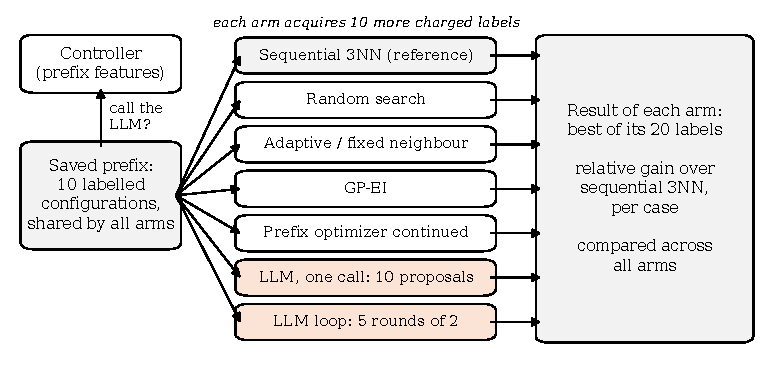
\includegraphics[width=\linewidth]{figures/design.pdf}
\caption{The paired-prefix design. Every arm starts from the same saved ten-label prefix and acquires ten more labels, each charged against the budget. An arm's result is the best of its 20 labels, compared per case with sequential 3NN and with the other arms. A controller sees only the prefix and decides once whether to call the LLM.}
\label{fig:design}
\end{figure}

Each continuation clones the prefix and acquires ten further configurations it has not seen, for a total of 20 labels. A continuation never sees another continuation's labels or any value it has not acquired. The candidate feature table is visible (the setting is transductive), but objective values are revealed only through a charged oracle. A continuation's result is the best value among its 20 labels.

The native cohort uses the same ten-label prefix. The remaining budget is seven search evaluations plus three fresh measurements of the selected configuration, whose median is the reported result. All selected configurations, including those of older runs, were re-measured together in randomized blocks, so every comparison uses measurements from the same session.

\subsection{Classical continuations}

From each prefix we ran several cheap continuations. The \emph{reference continuation} is \emph{sequential 3NN}. For each unmeasured configuration it predicts the objective as the mean of the three nearest measured configurations, measures the configuration with the best prediction, and repeats. Distance is Hamming distance for symbolic features, and mean normalized numeric difference plus category mismatch for Spark and Hadoop. Ties go to the earlier configuration in the case's seeded candidate order. For Spark and Hadoop this is also the optimizer that built the prefix; for the other six families it is not, so we also continued the \emph{prefix optimizer} itself, the full-domain centroid search.

The other continuations are simpler. An \emph{adaptive neighbour} rule measures the unmeasured configuration nearest to the current best, and a \emph{fixed neighbour} rule measures the configuration nearest to the prefix's best. \emph{Random} search draws uniformly from the unmeasured configurations. Gaussian-process expected improvement (\emph{GP-EI}) \cite{jones1998ego} uses a fixed mixed Mat\'ern-5/2 and Hamming kernel, with targets normalized using acquired labels only. For Spark and Hadoop we also ran \emph{random prototypes}: random proposals written in the LLM's proposal format and mapped to configurations by the same projection the LLM uses, which helps separate the effect of the projection from that of the model. On the native systems we also ran the acquisition functions of EZR version 0.9.4, unmodified (the centroid and naive-Bayes variants), through a thin wrapper that injects the saved prefix \cite{menzies2026ezr}.

\subsection{LLM continuations}

\paragraph{Models.} We used three local models in 4-bit quantization (Q4\_K\_M), served with llama.cpp \cite{gerganov2023llamacpp}: SmolLM3-3B \cite{huggingface2025smollm3}, Qwen3-8B and Qwen3-14B \cite{qwen2025qwen3}. Thinking mode was off, the temperature was 0.7 and top-$p$ was 0.95. In the final experiment we added gpt-oss-120b \cite{openai2025gptoss}, the model used by SNAP2, accessed through OpenRouter \cite{openrouter2025}. Reasoning effort was set to medium, a single serving provider handled all scientific requests, and output was capped at 16,000 tokens per one-shot call and 8,000 per loop call.

\paragraph{One-shot interface.} The model receives the feature names and their allowed values, the ten measured configurations with their objective values, and the direction of optimization. It is asked for ten new configurations, written as fixed-width symbol strings. Local decoding is constrained by a grammar, and hosted decoding by an equivalent JSON schema. Each proposal is projected to the nearest configuration not yet measured, using the reference's distance and tie-breaking. In the native cohort, where only seven search evaluations remain, the first seven proposals are used and projection uses ordinal distance. A malformed or truncated response triggers the reference continuation as a fallback, and the fallback's result is charged to the LLM arm.

\paragraph{Iterative loop.} To stay close to SNAP2 we also ran gpt-oss-120b in a loop of five rounds with two proposals per round. Each prompt repeats the original task description and the hard constraints on allowed symbols, lists every configuration measured so far from worst to best, and names earlier proposals that collided with already-measured configurations. On a retry it also gives the reason the previous answer was rejected. Each round allows one retry. A round that still fails falls back to the classical rule.

\subsection{Measures}

For a case with reference result $y_{\mathrm{ref}}$ and continuation result $y$, the relative gain is
\[
g = \frac{y_{\mathrm{ref}} - y}{y_{\mathrm{ref}}}
\]
when lower is better, with the sign reversed for throughput. Positive values favour the continuation. Because relative gains are asymmetric, we also report the log-ratio $\ell = \ln(y_{\mathrm{ref}}/y)$ ($\ln(y/y_{\mathrm{ref}})$ for throughput), aggregated in the same way as $g$. We call a case \emph{useful} if $g > 1\%$.

\paragraph{Aggregation.} The primary average weights each of the seven ecosystems equally: we average cases within an ecosystem, then average the seven ecosystem means. Without this, Spark and Hadoop would contribute 40 of the 70 cases. As sensitivity analyses we also report averages with equal weight per engine (eight groups) and per case, the primary average without DUNE, and the range of the primary average when each ecosystem is left out in turn.

\paragraph{Three comparisons for attribution.} Our results depend on what an LLM continuation is compared with, so we report three comparisons. The first is against the fixed reference, sequential 3NN, which is a deployable default.

The second is against a \emph{deployable classical policy}: for each held-out ecosystem, the classical continuation with the best primary average on the other six ecosystems. The choice uses only those training ecosystems, so nothing guarantees that the policy beats the fixed reference; we report its own gain relative to the reference alongside the comparison.

The third is against the \emph{best classical outcome in hindsight}. We call a case a \emph{baseline-set win} if the LLM continuation beats each member of a prespecified baseline set (sequential 3NN, random search, the adaptive neighbour rule and GP-EI) by more than 1\%. This asks whether any tested cheap method came within 1\% of the LLM's outcome, not whether a practitioner could have picked that method in advance. Beating these baselines does not by itself show that the LLM contributed something no other method could. We therefore also report an extended set that adds the fixed neighbour rule, the prefix optimizer and, where it was run, random prototypes.

\paragraph{Headroom.} We report \emph{hindsight headroom}, the mean of $\max(0, g)$. It is an empirical upper bound, for the recorded branch outcomes, on what choosing between that continuation and the reference could have gained. It is not a deployable policy, and it does not bound what other model draws or interaction designs might achieve.

\paragraph{Robust native wins.} On the native systems a win counts as robust only if the gain exceeds 10\%, the configuration differs from the reference's, quality is valid, the repeated measurements are stable (relative median absolute deviation of at most 5\%), and the medians are at least 10\,ms.

We do not run significance tests. Statistical tests are standard practice for comparing randomized algorithms in software engineering \cite{arcuri2011practical}, but they treat the compared runs as samples from a population. With seven groups, one of them holding 40 of the 70 cases, such tests would rest on strong assumptions about how the groups were sampled. We report the weighting and leave-one-out sensitivities and the variation between repeated model draws instead.

\subsection{Controllers}

All controllers decide once, after the prefix, using only 18 features available at that point. They describe the size of the problem (the number of candidates and options), the spread of the observed labels, the progress made between early and late prefix steps, the length of any plateau, and a bootstrap estimate of how stable the incumbent is.

We trained four fixed benefit predictors on the paired gains relative to the reference: ridge regression on 7 or 18 features, a depth-2 regression tree, and RBF kernel ridge. Evaluation used nested leave-one-group-out cross-validation. Scaling, model fitting and the decision threshold were chosen on inner folds that exclude the held-out group, and a meta-selection step picks one predictor per fold. We also report each predictor with a fixed 80th-percentile threshold, and a bootstrap-uncertainty rule. Two further rules adapt published methods to a single decision: a BORA-inspired rule that calls the LLM when a GP is uncertain or the search has plateaued \cite{cisse2025bora}, and an LB-MCTS-inspired rule that calls it with a probability derived from the surrogate's cross-validated rank reliability \cite{xu2026lbmcts}. These are adaptations, not the full iterative algorithms.

The controllers in Table~\ref{tab:rq4} were developed on the 3B and 8B paired data. Earlier versions of the benefit and uncertainty controllers were frozen and applied, unchanged, to systems as they were added during the study: one fitted on earlier development data was applied to WavPack and FFTW, and one fitted on seven families was applied to Hadoop. The controllers of Table~\ref{tab:rq4} were then applied, unchanged, to Memcached and the six native systems. After the final experiment we also reran their code, unchanged, on the Qwen3-14B and gpt-oss-120b gains. That rerun is exploratory.

\subsection{How the study evolved}
\label{sec:history}

The study went through many numbered iterations on the same systems, changing prompts, output formats, datasets, budgets and controllers along the way. Every protocol, raw model response, acquisition log and failure was kept in the project archive. The review package (see Data Availability) contains the protocols and freeze records of every iteration, and the records needed to reproduce the results reported here. Because the earlier analyses were carried out on data we had already seen, we treat them as exploratory.

The last two experiments were run differently: a test of Qwen3-14B against a repeated Qwen3-8B draw, and a test of gpt-oss-120b in the one-shot and loop interfaces. Both were prospectively frozen experiments on systems we had studied before, not confirmatory evaluations on untouched systems. Before any data were collected for each, we wrote a timestamped protocol file that fixed the code, the inputs (by content hash) and a decision rule. These files are kept in the replication package and were not registered with an external registry.

Every deviation was logged, with its time, before any outcome was scored. There were three: a failed server start that sent no requests; an output cap too small for a reasoning model, which surfaced together with provider rate limits; and wall-clock limits on individual stages. The repeated Qwen3-8B draw hit its pre-declared memory cap and completed only 45 of its 70 cases. We use it only as a check on sampling variability.

The analyses in Tables~\ref{tab:weights}, \ref{tab:deployable}, \ref{tab:match} and \ref{tab:routers-strong}, the extended baseline set and the reweighting of controller decisions were added after the outcomes were known.

\section{Results}

\subsection{\RQ{1}: Does the LLM continuation beat the reference?}
\label{sec:rq1}

Under the primary, ecosystem-balanced average, no (Table~\ref{tab:rq1}). Every LLM arm has a negative mean gain relative to sequential 3NN, from $-3.1\%$ for gpt-oss-120b in the loop to $-5.2\%$ for Qwen3-8B, and the log-ratio agrees in sign for every arm. The cheap classical alternatives also trail the reference, but by less. GP-EI is the strongest of them, with 22 cases more than 1\% better than the reference and 11 more than 1\% worse.

Figure~\ref{fig:cases} shows the individual cases behind these averages. Most gains above 1\% come from Spark and Hadoop: 98 of the 115 useful arm--case pairs across the nine continuations. Most losses beyond 30\% come from DUNE (17 of 21).

\begin{figure}[t]
\centering
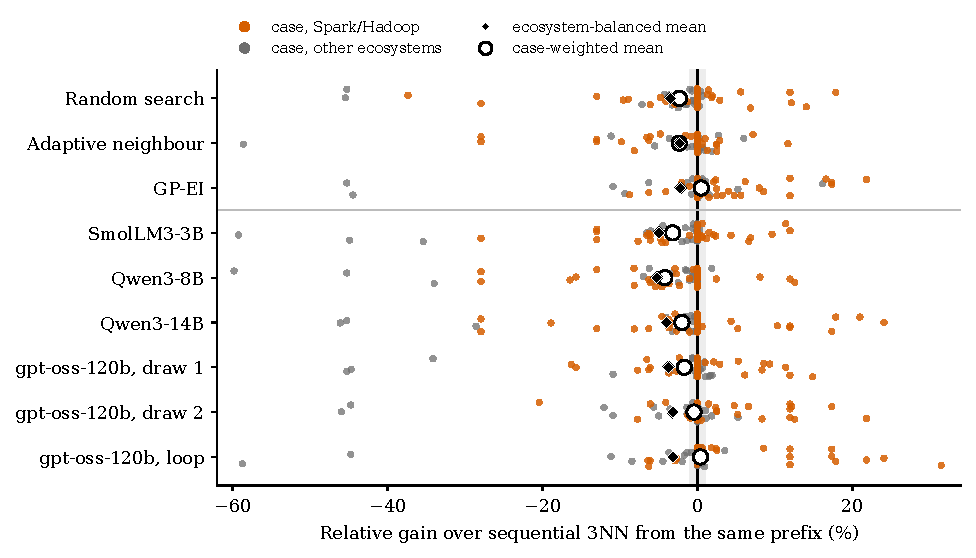
\includegraphics[width=\linewidth]{figures/case_gains.pdf}
\caption{Relative gain over sequential 3NN for every case of the recorded cohort, by continuation (70 points per row, jittered vertically). The grey band marks $\pm1\%$. Diamonds give the ecosystem-balanced mean reported in Table~\ref{tab:rq1}; circles give the case-weighted mean, which Spark and Hadoop dominate.}
\label{fig:cases}
\end{figure}

\begin{table}[t]
\centering
\caption{\RQ{1}, recorded cohort (70 cases; primary average with the seven ecosystems weighted equally). Gains are relative to sequential 3NN from the same prefix. ``Better'' and ``worse'' count cases more than 1\% above and below the reference. Headroom is the mean of $\max(0,g)$.}
\label{tab:rq1}
\small
\begin{tabular}{lrrrrr}
\toprule
Continuation & Mean gain & Log-ratio & Better & Worse & Headroom \\
\midrule
Random search & $-3.49\%$ & $-2.97\%$ & 11 & 22 & 0.32\% \\
Adaptive neighbour & $-2.29\%$ & $-1.90\%$ & 10 & 17 & 0.48\% \\
GP-EI & $-2.19\%$ & $-1.66\%$ & 22 & 11 & 1.28\% \\
\midrule
SmolLM3-3B & $-4.96\%$ & $-4.56\%$ & 10 & 24 & 0.22\% \\
Qwen3-8B & $-5.24\%$ & $-4.79\%$ & 5 & 29 & 0.18\% \\
Qwen3-14B & $-4.00\%$ & $-3.60\%$ & 9 & 23 & 0.45\% \\
gpt-oss-120b, one-shot, draw 1 & $-3.73\%$ & $-3.48\%$ & 15 & 14 & 0.52\% \\
gpt-oss-120b, one-shot, draw 2 & $-3.16\%$ & $-2.69\%$ & 19 & 15 & 0.76\% \\
gpt-oss-120b, iterative loop & $-3.14\%$ & $-2.48\%$ & 14 & 14 & 0.86\% \\
\bottomrule
\end{tabular}
\end{table}

The ecosystem means differ widely (Table~\ref{tab:eco}). DUNE is hard for every continuation: each one in Table~\ref{tab:eco} has a mean loss of more than 11\% relative to the reference. OpenVPN hurts four of the six LLM arms by 5.9--9.0\%, against 1--2\% for the classical alternatives. Spark and Hadoop form the only ecosystem where several LLM arms gain more than 2\% on average, and GP-EI gains there too. Elsewhere, LLM gains, where they occur at all, stay below about 1\%.

\begin{table}[t]
\centering
\caption{Mean gain relative to sequential 3NN by ecosystem (recorded cohort). The Spark/Hadoop row averages 40 cases; every other row averages 5.}
\label{tab:eco}
\small
\setlength{\tabcolsep}{4pt}
\begin{tabular}{lrrrrrrrrr}
\toprule
 & \multicolumn{3}{c}{Classical} & \multicolumn{3}{c}{Local LLM} & \multicolumn{3}{c}{gpt-oss-120b} \\
\cmidrule(lr){2-4}\cmidrule(lr){5-7}\cmidrule(lr){8-10}
Ecosystem & Random & Adapt. & GP-EI & 3B & 8B & 14B & Draw 1 & Draw 2 & Loop \\
\midrule
BerkeleyDB & $-1.04$ & $+0.71$ & $+4.51$ & $-0.33$ & $+0.06$ & $-0.87$ & $-0.34$ & $+0.92$ & $+0.21$ \\
DUNE & $-18.14$ & $-11.15$ & $-18.06$ & $-20.89$ & $-21.24$ & $-18.61$ & $-18.01$ & $-18.38$ & $-20.63$ \\
HIPAcc & $-0.64$ & $-0.71$ & $-1.06$ & $-2.60$ & $-2.91$ & $-1.37$ & $+1.03$ & $-0.89$ & $-1.61$ \\
LLVM & $-2.20$ & $+0.14$ & $-1.61$ & $-1.97$ & $-2.16$ & $-1.00$ & $-0.01$ & $-1.07$ & $-1.62$ \\
OpenVPN & $-0.97$ & $-2.23$ & $-2.19$ & $-7.08$ & $-6.88$ & $-5.87$ & $-9.00$ & $-4.59$ & $-2.38$ \\
SaC & $-0.27$ & $-0.40$ & $-0.14$ & $-0.40$ & $-0.40$ & $-0.27$ & $-0.14$ & $-0.40$ & $+0.13$ \\
Spark/Hadoop & $-1.15$ & $-2.41$ & $+3.18$ & $-1.42$ & $-3.16$ & $+0.01$ & $+0.37$ & $+2.29$ & $+3.93$ \\
\bottomrule
\end{tabular}
\end{table}

\paragraph{Sensitivity to weighting.} The primary average is sensitive to weighting and to DUNE (Table~\ref{tab:weights}). Every LLM arm still trails the reference under equal weight per engine, and in every leave-one-ecosystem-out average. Under equal weight per case, which lets Spark and Hadoop dominate, the gpt-oss-120b loop gains 0.40\% (log-ratio $+0.99\%$). GP-EI gains a similar 0.49\% under the same case weighting, while the one-shot gpt-oss-120b draws and the local models still trail. The statement ``every model lost on average'' therefore holds for the prespecified ecosystem-balanced average, and not for every reasonable weighting.

\begin{table}[t]
\centering
\caption{Sensitivity of the mean gain relative to sequential 3NN to weighting (recorded cohort; percent). LOEO: range of the primary average when each ecosystem is left out in turn. Post hoc.}
\label{tab:weights}
\small
\begin{tabular}{lrrrrr}
\toprule
Continuation & Ecosystem & Engine & Case & Excl.\ DUNE & LOEO range \\
\midrule
Random search & $-3.49$ & $-3.25$ & $-2.32$ & $-1.05$ & $[-4.02, -1.05]$ \\
Adaptive neighbour & $-2.29$ & $-2.53$ & $-2.35$ & $-0.82$ & $[-2.79, -0.82]$ \\
GP-EI & $-2.19$ & $-1.39$ & $+0.49$ & $+0.45$ & $[-3.31, +0.45]$ \\
Prefix optimizer continued & $-2.25$ & $-1.97$ & $-1.12$ & $-1.13$ & $[-2.75, -1.13]$ \\
\midrule
SmolLM3-3B & $-4.96$ & $-4.62$ & $-3.19$ & $-2.30$ & $[-5.73, -2.30]$ \\
Qwen3-8B & $-5.24$ & $-5.09$ & $-4.20$ & $-2.57$ & $[-6.12, -2.57]$ \\
Qwen3-14B & $-4.00$ & $-3.63$ & $-1.99$ & $-1.56$ & $[-4.66, -1.56]$ \\
gpt-oss-120b, draw 1 & $-3.73$ & $-3.18$ & $-1.68$ & $-1.35$ & $[-4.52, -1.35]$ \\
gpt-oss-120b, draw 2 & $-3.16$ & $-2.32$ & $-0.43$ & $-0.62$ & $[-4.07, -0.62]$ \\
gpt-oss-120b, loop & $-3.14$ & $-2.16$ & $+0.40$ & $-0.22$ & $[-4.32, -0.22]$ \\
\bottomrule
\end{tabular}
\end{table}

\paragraph{Native cohort.} The native cohort shows the same pattern for SmolLM3-3B and Qwen3-8B (Table~\ref{tab:native}). On OR-Tools and XGBoost the LLM continuations lose by 20--26\%, while on cvc5, ripgrep and hnswlib the differences are within a few percent. For each model, the LLM chose exactly the reference's configuration in 17 of the 30 cases, and no continuation, classical or LLM, produced a robust win over the reference. The native cohort therefore did not demonstrate robust improvements over the reference for any method. That is not the same as showing that nothing was left to find.

We measured every configuration of two of the systems exhaustively, for offline analysis only, and selected the best one. For hnswlib, the selected configuration was not faster on fresh measurements than the prefix incumbent in any seed. For ripgrep it was: 5.3\% faster on average and up to 12.7\% in one seed, with one seed clearing the robust threshold. No continuation found it robustly. So the absence of wins on ripgrep reflects a failure to find an available improvement, while on hnswlib there was little to find.

\begin{table}[t]
\centering
\caption{Native cohort: mean gain relative to sequential 3NN (five seeds each; medians of three fresh measurements taken in the same session). No arm, classical or LLM, has a robust win on any system.}
\label{tab:native}
\small
\begin{tabular}{lrrr}
\toprule
System & SmolLM3-3B & Qwen3-8B & Robust wins (any arm) \\
\midrule
cvc5 (N-queens) & $-0.11\%$ & $+0.16\%$ & 0 \\
OR-Tools CP-SAT (N-queens) & $-20.67\%$ & $-20.22\%$ & 0 \\
ripgrep & $-2.17\%$ & $-0.32\%$ & 0 \\
hnswlib & $-0.15\%$ & $-0.24\%$ & 0 \\
Polars & $-5.07\%$ & $-4.83\%$ & 0 \\
XGBoost & $-26.11\%$ & $-19.53\%$ & 0 \\
\bottomrule
\end{tabular}
\end{table}

\subsection{\RQ{2}: Would a cheap classical alternative have done as well?}
\label{sec:rq2}

The answer depends on which of the three comparisons we use.

\paragraph{Against a deployable classical policy.} Table~\ref{tab:deployable} compares each LLM arm with the classical continuation chosen using only the other six ecosystems. That choice was sequential 3NN in six folds and GP-EI in one, the fold in which DUNE was held out. The policy itself did worse than the fixed reference: $-2.58\%$ under the primary average and $-1.29\%$ per case. Its only switch, to GP-EI on DUNE, lost about 45\% in two of the five DUNE cases and was never more than 1\% better than the reference.

The local models still trail this policy clearly. gpt-oss-120b comes closer, between $-0.44\%$ and $-1.15\%$ under the primary average, but most of that narrowing reflects the policy's own loss on DUNE rather than any gain by the LLM. Under case weighting its second draw and loop are ahead of the policy, by 0.86\% and 1.75\%. Against the fixed reference the same arms gain $-0.43\%$ and $+0.40\%$, so again most of the difference comes from the policy's DUNE loss.

\begin{table}[t]
\centering
\caption{Each LLM arm against a deployable classical policy chosen by leave-one-ecosystem-out (the classical continuation with the best primary average on the other ecosystems). The first row gives the policy itself relative to sequential 3NN; the other rows give each LLM arm relative to the policy. ``Better'' and ``worse'' count cases beyond 1\%. Post hoc.}
\label{tab:deployable}
\small
\begin{tabular}{lrrrr}
\toprule
Comparison & Ecosystem-balanced & Case-weighted & Better & Worse \\
\midrule
Policy vs.\ sequential 3NN & $-2.58\%$ & $-1.29\%$ & 0 & 2 \\
\midrule
SmolLM3-3B & $-2.25\%$ & $-1.83\%$ & 10 & 23 \\
Qwen3-8B & $-2.53\%$ & $-2.84\%$ & 5 & 27 \\
Qwen3-14B & $-1.40\%$ & $-0.70\%$ & 9 & 21 \\
gpt-oss-120b, draw 1 & $-1.15\%$ & $-0.39\%$ & 15 & 12 \\
gpt-oss-120b, draw 2 & $-0.57\%$ & $+0.86\%$ & 19 & 13 \\
gpt-oss-120b, loop & $-0.44\%$ & $+1.75\%$ & 14 & 13 \\
\bottomrule
\end{tabular}
\end{table}

\paragraph{Against the best classical outcome in hindsight.} Table~\ref{tab:match} takes every case in which an LLM arm beat the reference by more than 1\% and asks how the best of the three prespecified cheap alternatives (random search, the adaptive neighbour rule and GP-EI) did on the same prefix. In 61 of the 72 arm--case pairs, at least one alternative reached a result as good as the LLM's or better, and in 3 more the best alternative came within 1\% of the LLM. The remaining 8 are the baseline-set wins counted in Table~\ref{tab:rq2}; none of them belongs to the 3B or 8B model. Random search alone has 11 useful cases, against 10 for SmolLM3-3B and 5 for Qwen3-8B (Table~\ref{tab:rq1}). In Spark and Hadoop, random prototypes passed through the LLM's own projection beat the reference on average (+1.17\% on Spark, +4.42\% on Hadoop), whereas SmolLM3-3B's proposals did worse there ($-0.11\%$ and $-3.60\%$). Most LLM wins over the reference therefore came on prefixes where a cheap alternative did at least as well.

\begin{table}[t]
\centering
\caption{Cases in which an LLM arm beat sequential 3NN by more than 1\% (``useful''), classified by how the best of random search, the adaptive neighbour rule and GP-EI did on the same prefix. ``At least as good'': that alternative's result equals or beats the LLM's. ``Within 1\%'': the LLM is ahead by at most 1\%. ``LLM ahead'': the LLM beats every alternative by more than 1\%, which is a baseline-set win. Post hoc.}
\label{tab:match}
\small
\begin{tabular}{lrrrrr}
\toprule
LLM arm & Useful cases & Ecosystems & At least as good & Within 1\% & LLM ahead \\
\midrule
SmolLM3-3B & 10 & 1 & 10 & 0 & 0 \\
Qwen3-8B & 5 & 2 & 4 & 1 & 0 \\
Qwen3-14B & 9 & 1 & 7 & 0 & 2 \\
gpt-oss-120b, draw 1 & 15 & 3 & 11 & 1 & 3 \\
gpt-oss-120b, draw 2 & 19 & 3 & 17 & 1 & 1 \\
gpt-oss-120b, loop & 14 & 2 & 12 & 0 & 2 \\
\midrule
Total & 72 & -- & 61 & 3 & 8 \\
\bottomrule
\end{tabular}
\end{table}

Table~\ref{tab:rq2} counts baseline-set wins, with their denominators within each ecosystem. SmolLM3-3B and Qwen3-8B had none. Qwen3-14B had two, both on Spark; with the extended baseline set only one remains, because random prototypes reached the other. The gpt-oss-120b wins are unchanged by the extended set. In the native cohort, neither the 3B nor the 8B model had a case that beat every classical alternative by more than 1\%, and native hindsight headroom was 0.36\% and 0.40\% for the two models, barely above random search's 0.30\% and less than half that of EZR's naive-Bayes acquisition (0.90\%).

\begin{table}[t]
\centering
\caption{\RQ{2}--\RQ{3}: baseline-set wins in the recorded cohort. A win beats sequential 3NN, random search, the adaptive neighbour rule and GP-EI each by more than 1\%. Cells give wins over cases within the ecosystem. ``Extended'' adds the fixed neighbour rule, the prefix optimizer and, for Spark and Hadoop, random prototypes (post hoc).}
\label{tab:rq2}
\small
\begin{tabular}{lcccrr}
\toprule
 & \multicolumn{3}{c}{Wins by ecosystem} & & \\
\cmidrule(lr){2-4}
LLM arm & HIPAcc & Spark/Hadoop & Others & Ecosystems & Extended \\
\midrule
SmolLM3-3B & 0/5 & 0/40 & 0/25 & 0 & 0 \\
Qwen3-8B & 0/5 & 0/40 & 0/25 & 0 & 0 \\
Qwen3-14B & 0/5 & 2/40 & 0/25 & 1 & 1 (1 case) \\
gpt-oss-120b, draw 1 & 2/5 & 1/40 & 0/25 & 2 & 2 (3 cases) \\
gpt-oss-120b, draw 2 & 0/5 & 1/40 & 0/25 & 1 & 1 (1 case) \\
gpt-oss-120b, loop & 0/5 & 2/40 & 0/25 & 1 & 1 (2 cases) \\
\bottomrule
\end{tabular}
\end{table}

\subsection{\RQ{3}: Do stronger models or iterative interaction help?}
\label{sec:rq3}

The stronger models did better, but our design does not separate model size from the other differences between arms. The local models ran quantized with thinking disabled and one-shot, while gpt-oss-120b used medium reasoning effort.

\paragraph{Qwen3-8B to Qwen3-14B.} Prompts and seeds were unchanged, and the rendered prompts were identical byte for byte. The primary mean loss fell from 5.24\% to 4.00\%, and Qwen3-14B was more than 1\% better than the earlier 8B draw in 16 cases and worse in 5.

\paragraph{gpt-oss-120b.} Its first one-shot draw was more than 1\% better than Qwen3-8B in 27 cases and worse in 5. Before collecting its data we fixed a decision rule: baseline-set wins in at least two of the seven ecosystems, in either the first one-shot draw or the loop, would count as evidence of headroom at this model scale.

The first draw met the rule exactly (Table~\ref{tab:rq2}), but the result is fragile. The two HIPAcc cases that supplied the second ecosystem won by only 1.9\% and 1.7\%, and did not recur: in the second draw they scored $-5.6\%$ and 0.0\%, and in the loop $-1.7\%$ and $-2.0\%$. The second draw and the loop each reached one ecosystem. When we raised the margin to 2\% after seeing the data, or separately required a win to appear in at least two of the three runs, every run fell to one ecosystem, Spark/Hadoop.

\paragraph{Variation between draws.} This is part of the result, not a side note. Two draws of gpt-oss-120b on identical prompts and prefixes disagreed by more than 1\% in 26 of 70 cases (Figure~\ref{fig:draws}, left). Only one task--prefix pair produced a baseline-set win in all three gpt-oss-120b runs: the Spark Bayes workload with seed 11. It beat the reference by 8.3\% in both one-shot draws and by 31.5\% in the loop, where it also beat GP-EI by 27\%. None of the local models beat the reference on it. This is one prefix

\begin{figure}[t]
\centering
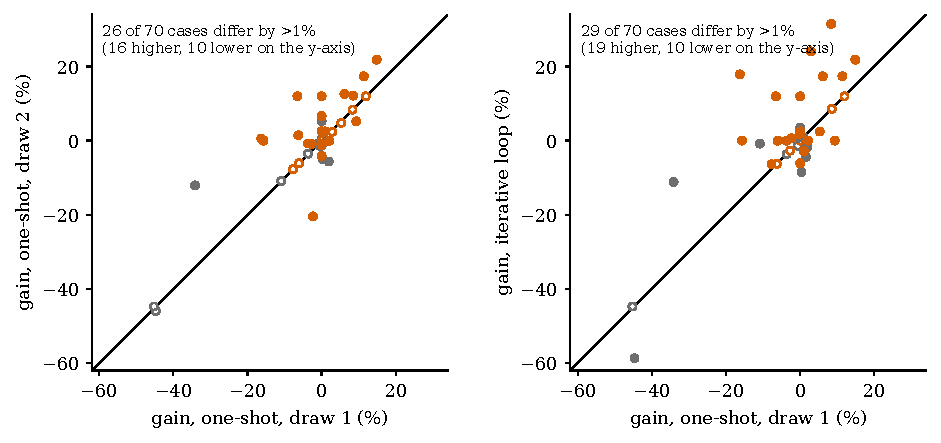
\includegraphics[width=\linewidth]{figures/draw_variability.pdf}
\caption{Case-by-case gains of gpt-oss-120b over sequential 3NN on identical prefixes. Left: the two one-shot draws. Right: the first one-shot draw against the iterative loop. Filled points are cases where the two results differ by more than 1\%; hollow points agree within 1\%. Orange marks Spark and Hadoop cases.}
\label{fig:draws}
\end{figure}
 of one task, repeated three times, not replication across systems. In a second Spark case (TeraSort, seed 23) the loop matched a 24\% gain that Qwen3-14B had also found.

\paragraph{The iterative loop.} The loop produced the largest single-case gain, the highest hindsight headroom (0.86\%) and the best case-weighted mean of any LLM arm. Its primary mean ($-3.14\%$) is, however, almost identical to the second one-shot draw's ($-3.16\%$). Its advantage over the first draw (19 cases better and 10 worse) is of the same order as the disagreement between two one-shot draws (Figure~\ref{fig:draws}, right). An earlier exploratory experiment with Qwen3-8B on LLVM and SaC also compared five rounds of measured feedback with a control in which the feedback was masked; the two ended with the same incumbent in all ten cases. Repeated, matched one-shot and loop runs on identical prefixes would be needed to separate an interaction effect from inference variability.

\subsection{\RQ{4}: Does a controller improve on never calling?}
\label{sec:rq4}

On the recorded cohort, none of the controllers we evaluated did so by as much as 0.03 percentage points, under the primary average or under engine or case weighting. Table~\ref{tab:rq4} shows them under the primary average for the two models on which they were developed. On the native systems, one transferred rule did better than never calling by 0.15\%, from a single call (see below).

\begin{table}[t]
\centering
\caption{\RQ{4}: controllers under leave-one-ecosystem-out evaluation for the models they were developed on (70 cases each; primary ecosystem-balanced average). Gains are relative to sequential 3NN and are zero for any case in which the controller does not call the LLM. The oracle picks the better branch after seeing both outcomes and is not deployable.}
\label{tab:rq4}
\small
\begin{tabular}{lrrrr}
\toprule
 & \multicolumn{2}{c}{Calls (of 70)} & \multicolumn{2}{c}{Mean gain} \\
\cmidrule(lr){2-3}\cmidrule(lr){4-5}
Policy & SmolLM3 & Qwen3-8B & SmolLM3 & Qwen3-8B \\
\midrule
Never call & 0 & 0 & $0.00\%$ & $0.00\%$ \\
Always call & 70 & 70 & $-4.96\%$ & $-5.24\%$ \\
Benefit predictor (inner-CV selection) & 0 & 0 & $0.00\%$ & $0.00\%$ \\
Ridge, 18 features, 80th percentile & 9 & 9 & $-0.10\%$ & $-0.10\%$ \\
Regression tree, 80th percentile & 4 & 8 & $-2.97\%$ & $-0.45\%$ \\
Bootstrap uncertainty, 80th percentile & 27 & 27 & $-3.12\%$ & $-3.16\%$ \\
BORA-inspired checkpoint rule & 14 & 14 & $-3.10\%$ & $-3.25\%$ \\
Rank-reliability rule (expected calls) & 23.95 & 23.95 & $-1.44\%$ & $-1.49\%$ \\
\midrule
Hindsight oracle & -- & -- & $+0.22\%$ & $+0.18\%$ \\
\bottomrule
\end{tabular}
\end{table}

\paragraph{Small models.} With the threshold chosen on inner folds, the benefit predictor never called the LLM. The frozen benefit controllers applied to later systems also made no calls: the earlier versions on WavPack, FFTW and Hadoop, and the version in Table~\ref{tab:rq4} on Memcached and the six native systems. The rules that did call the LLM lost, and the uncertainty, BORA-inspired and rank-reliability rules also did worse than calls chosen at random at the same rate. In the native cohort the two adapted rules made between 1 and 7 calls per ten cases. Their outcomes, relative to never calling, ranged from a gain of 0.15\% (from a single call) to a loss of 7.5\%.

\paragraph{Why the small-model data are hard to learn from.} For SmolLM3-3B all ten gains above 1\% fall in the Spark/Hadoop ecosystem. Holding that ecosystem out therefore leaves no above-threshold examples in training, and holding out any other ecosystem leaves none in the test fold. Qwen3-8B has such gains in two ecosystems. This concerns the 1\% threshold only. The predictors are trained on continuous gains, and smaller positive gains occur in other ecosystems, so these data limit, but do not rule out, what a predictor could learn.

\paragraph{Stronger models (rerun, exploratory).} The stronger arms offer more to learn from: gpt-oss-120b has gains above 1\% in two or three ecosystems. Table~\ref{tab:routers-strong} reruns the same controller code, unchanged. The selected benefit predictor made no calls for Qwen3-14B; for the gpt-oss-120b arms it made 3 to 5 calls and lost between 0.06\% and 2.95\%. The best fixed-quantile rule for each arm ended between 0.04 percentage points below and 0.02 above never calling. A few rules did better than calls chosen at random at the same rate, but none improved on never calling by as much as 0.03 percentage points. Hindsight headroom for these arms is 0.45--0.86\%, so even a perfect choice between each arm and the reference would have gained little on average.

\paragraph{Other weightings.} A controller's held-out decisions are fixed per case, so we can reweight its outcomes without retraining anything. Tables~\ref{tab:rq4} and~\ref{tab:routers-strong} use the primary average. Across all six arms, the best controller exceeded never calling by at most 0.019 percentage points under engine weighting and 0.011 under case weighting. The BORA-inspired and rank-reliability rules, evaluated only on the 3B and 8B models, lost under every weighting (for example $-1.96\%$ and $-0.83\%$ for SmolLM3-3B under case weighting). Case weighting does change one comparison. For the iterative gpt-oss-120b arm, always calling gains 0.40\% under that weighting, so there the relevant trivial baseline is always calling, and every controller falls short of it by about 0.39 percentage points or more.

\begin{table}[t]
\centering
\caption{The same controllers rerun post hoc on the stronger arms (leave-one-ecosystem-out; primary ecosystem-balanced mean gain relative to sequential 3NN, with calls in parentheses). ``Groups'' counts ecosystems with at least one gain above 1\%.}
\label{tab:routers-strong}
\small
\setlength{\tabcolsep}{4pt}
\begin{tabular}{lrrrrr}
\toprule
LLM arm & Groups & Selected predictor & Ridge, 80th pct. & Uncertainty, 80th pct. & Oracle \\
\midrule
Qwen3-14B & 1 & $0.00\%$ (0) & $-0.16\%$ (9) & $-2.55\%$ (27) & $+0.45\%$ \\
gpt-oss-120b, draw 1 & 3 & $-1.30\%$ (3) & $-0.07\%$ (10) & $-2.51\%$ (27) & $+0.52\%$ \\
gpt-oss-120b, draw 2 & 3 & $-0.06\%$ (5) & $+0.02\%$ (9) & $-2.40\%$ (27) & $+0.76\%$ \\
gpt-oss-120b, loop & 2 & $-2.95\%$ (5) & $+0.02\%$ (9) & $-2.77\%$ (27) & $+0.86\%$ \\
\bottomrule
\end{tabular}
\end{table}

These results show that the controllers we evaluated did not reliably help on these cohorts, with these features and at this budget. They do not show that useful escalation routing is impossible. Sparse and concentrated gains limit how much any cross-system evaluation of that question can reveal.

\section{Discussion}

\subsection{What this means for practitioners}

With a budget of around 20 evaluations and after a classical warm-up, calling an LLM by default did not pay off in our data under the primary average. This held for the local models and for gpt-oss-120b. The picture changes with emphasis, though. If Spark-like big-data workloads dominate one's portfolio, the case-weighted results suggest that gpt-oss-120b in a loop and GP-EI both do about as well as or slightly better than the nearest-neighbour reference.

A cheap switch to another classical strategy is a serious competitor, but choosing it is not free. In most cases where an LLM beat the reference, some cheap classical alternative from the same prefix did at least as well. Knowing in advance which alternative to use is a separate problem: our simple leave-one-ecosystem-out selector switched to GP-EI once, on DUNE, where the switch hurt most.

\subsection{What this means for researchers}

\paragraph{Report all three comparisons.} Improvement over a fixed reference overstates the LLM's contribution when other cheap strategies would also have improved. The best classical outcome in hindsight overstates what a practitioner could have achieved. A classical policy chosen using only the training groups answers the practitioner's question, but it is not guaranteed to lie between the other two. Ours did worse than the fixed reference, so the LLM's gap to it looks smaller than its gap to the reference. We recommend reporting all three, with the selected policy's own result against the reference, together with random search, a neighbourhood rule and a Bayesian-optimization baseline from the same prefix and budget.

\paragraph{Check how gains are distributed before evaluating a router.} Leave-one-group-out evaluation of a router says little when positive cases are concentrated in one or two groups. Counting gains above the practical threshold in each group, alongside the continuous gains, should come before training a router. Then abstention can be interpreted correctly.

\paragraph{Averages hide rare gains, and draws vary.} gpt-oss-120b's mean gain was negative under the primary average in every run, yet it produced one large gain that no other method found. Its draws disagreed on more than a third of the cases. Studies of LLM escalation need several draws per prefix before rare gains can be distinguished from noise.

\subsection{Cost and reliability}

Table~\ref{tab:ops} reports the operational side of each arm. All 140 one-shot gpt-oss-120b calls eventually produced valid answers. Seventeen attempts were first rejected by the provider's rate limit (HTTP 429) before any generation; they were retried after a pause and incurred no reported charge. The loop planned 350 calls (70 cases, five rounds each) and made 13 retries, 363 calls in all. Fifteen of them were truncated at the 8,000-token cap. Of the 13 rounds that needed a retry, 11 recovered and 2 fell back to the classical rule.

Before the frozen run, a first attempt with a 4,000-token cap was stopped after 11 requests. It is not part of the results but is kept in the record: 2 responses were truncated, 8 requests were rate-limited, and 1 request was still in flight when the attempt was stopped. Recorded hosted spend was \$1.38 in total. The three analysed arms account for \$1.374, and the provider probes and the stopped first attempt for the remaining \$0.003. The cost of the one request in flight is unknown.
Proposal latency is only part of the cost of tuning. Where objective evaluations are expensive or a configuration is reused many times, a 30-second call matters little. The question is whether the call buys a better configuration, and under the primary ecosystem-balanced average in our data it did not.

\begin{table}[t]
\centering
\caption{Operational summary per LLM arm (recorded cohort). \emph{Planned}: calls the protocol requires (one per case one-shot, one per round in the loop). \emph{Retries}: extra calls after an invalid response (loop only). \emph{429}: attempts rejected by the provider's rate limit before generation, retried after a pause and not counted as calls. \emph{Invalid}: responses that failed validation. \emph{Fallbacks}: cases (one-shot) or rounds (loop) resolved by the classical rule. Latency is the mean time per successful call. Cost is the provider-reported charge; local runs were on an Apple M3 Pro laptop and have no charge.}
\label{tab:ops}
\small
\setlength{\tabcolsep}{4pt}
\begin{tabular}{lrrrrrrr}
\toprule
Arm & Planned & Retries & 429 & Invalid & Fallbacks & Latency & Cost \\
\midrule
SmolLM3-3B & 70 & 0 & -- & 1 (interrupted) & 1 case & 4.0\,s & -- \\
Qwen3-8B & 70 & 0 & -- & 0 & 0 & 15.3\,s & -- \\
Qwen3-14B & 70 & 0 & -- & 0 & 0 & 26.1\,s & -- \\
gpt-oss-120b, draw 1 & 70 & 0 & 14 & 0 & 0 & 32.3\,s & \$0.25 \\
gpt-oss-120b, draw 2 & 70 & 0 & 3 & 0 & 0 & 26.8\,s & \$0.24 \\
gpt-oss-120b, loop & 350 & 13 & 0 & 15 (truncated) & 2 rounds & 9.9\,s & \$0.89 \\
\bottomrule
\end{tabular}
\end{table}

\section{Threats to Validity}

\paragraph{Construct validity.} Relative gains are asymmetric, but the log-ratios agree in sign for the primary average. The 1\% margin is a choice, and post-hoc checks at 2\% and 5\% make the gpt-oss-120b result weaker, not stronger. A baseline-set win shows that no tested cheap method came within 1\% of the LLM; it does not isolate an LLM-specific mechanism. Recorded measurements are single runs with no noise estimate, although the native cohort, which has repeated measurements, shows the same pattern for the small models. For Hadoop, failed runs receive a fixed penalty rather than a measured runtime. The hosted model's weights cannot be verified by hash, so we recorded the provider, model identifier, response identifiers and token usage for every call. SNAP2 does not report its reasoning setting, so we chose medium effort in advance.

\paragraph{Internal validity.} Extensive adaptive development on the same systems limits any confirmatory reading of the earlier experiments \cite{gelman2014forking}. The last two experiments were frozen before collection, but on previously studied systems, and their protocol files are timestamped locally rather than registered externally. The repeated Qwen3-8B draw is incomplete, and hosted inference is not deterministic, even with fixed seeds. The weighting sensitivities, the deployable-policy comparison, the extended baselines, the matching analysis, the rerun of controllers on the stronger arms and their reweighting were all added after the outcomes were known. The deployable classical policy is one simple selector; a better selector could narrow or widen its gap to the LLM arms.

\paragraph{External validity.} Seven ecosystems is a small sample, and one of them supplies 40 of the 70 cases. The native systems have small configuration spaces and were run only with the 3B and 8B models. We used one budget and one hand-off point, all local runs used one laptop, and the hosted runs used one provider. All tasks use public data that may appear in the models' pretraining data. The results do not rule out benefit at other budgets, or with other models, interfaces or task distributions.

\paragraph{Conclusion validity.} We report descriptive results with weighting and leave-one-out sensitivities rather than significance tests. Seeds are repeated measurements of the same system, not independent observations. The disagreement between repeated draws shows that single-draw results for LLM arms should be read with caution.

\section{Conclusion}

Our setting was a fixed budget of 20 evaluations with a shared ten-evaluation prefix. Averaged with equal weight per ecosystem, the LLM continuations we evaluated did worse than sequential nearest-neighbour search. That average depends on weighting: per case, the iterative gpt-oss-120b arm was slightly ahead, much like Gaussian-process expected improvement. In most cases where an LLM beat the reference by more than 1\%, a prespecified cheap classical continuation did at least as well. The hosted iterative model produced a small number of larger improvements, but only one task--prefix pair achieved a baseline-set win in all three evaluated gpt-oss-120b arms.

On the recorded cohort, the controllers we evaluated did not beat the better of always and never calling the LLM by as much as 0.03 percentage points under any of our weightings, either for the small models they were developed on or for the stronger models when rerun. Under case weighting, always calling the iterative gpt-oss-120b arm did better than every controller. These findings argue for stronger classical controls and for checking where escalation gains occur before evaluating routers. They do not show that useful routing is impossible, or that escalating to an LLM lacks value under other budgets, interfaces or task distributions.

A natural next step has two parts: repeating the strongest model's one-shot and iterative arms on identical prefixes, with matched controls, and evaluating routing on a cohort of new systems whose inclusion criteria are fixed without reference to LLM outcomes.

\section*{Data Availability}

The replication package is available at \url{https://github.com/mayankdhingra02/when-is-an-llm-worth-calling}. It contains the protocols and timestamped freeze records for every iteration of the study. For the results reported in this paper it also contains the saved observations, raw model responses with token usage, acquisition logs and deviation logs, together with the analysis and independent verification scripts, a command that reproduces the reported results offline, and the project's original integrity manifests. Measurement tables from three third-party sources (DeepPerf, Tuneful and Performance Evolution) are not redistributed; a script in the package downloads them from their owners' repositories at the versions we used and checks each against its recorded hash. Raw records of earlier iterations that this paper does not report are kept in the project archive. The package's manifest lists each of them, with its recorded hash. Four raw re-validation checks need runtimes that the package does not include; its README lists them. Byte-identical outputs and exact replays of search trajectories are expected only with the Python and library versions the package pins. With other versions, floating-point differences can make exact-match checks fail, and can change near-tied selections in replays, although the recorded observations are unchanged. The package contains no model weights or API credentials.

\section*{Acknowledgements}

This work received no specific funding. The author used AI assistants in this project. Claude (Anthropic), through the Claude Code tool, helped design, implement and run the experiments and analyses, and drafted and revised the manuscript under the author's direction. ChatGPT (OpenAI) reviewed drafts of the manuscript and independently audited the replication package. The author takes full responsibility for the content of this paper.

\bibliographystyle{plainnat}
\bibliography{references}

\end{document}
